\chapter{Resultados y conclusiones}
%\addcontentsline{toc}{chapter}{Introduction}

\pagestyle{fancy}
\fancyhf{}
\fancyhead[LE]{\nouppercase{\textbf{\leftmark}\hfill\textit{\rightmark}}}
\fancyhead[RO]{\nouppercase{\textit{\rightmark}\hfill\textbf{\leftmark}}}
\fancyfoot[LE]{\nouppercase{\thepage\hfill Pressure Distribution Inside Nucleons in a Tsallis-MIT Bag Model}}
\fancyfoot[RO]{\nouppercase{Pressure Distribution Inside Nucleons in a Tsallis-MIT Bag Model \hfill \thepage}}

\section{Comparación con resultados de Lattice QCD}

La figura~\ref{fig:Results_LQCD} compara las distribuciones de presión radial \( r^2 P(r) \) obtenidas con el modelo Tsallis-MIT para distintos valores del potencial químico \( \mu \), con los resultados recientes de Lattice QCD reportados por Shanahan y Detmold~\cite{shanahanPressureDistributionShear2019}. Las curvas continuas representan nuestras predicciones, mientras que los puntos corresponden a distribuciones extraídas numéricamente mediante simulaciones de QCD en el retículo.

\begin{wrapfigure}{o}{0.58\textwidth}
    \centering
    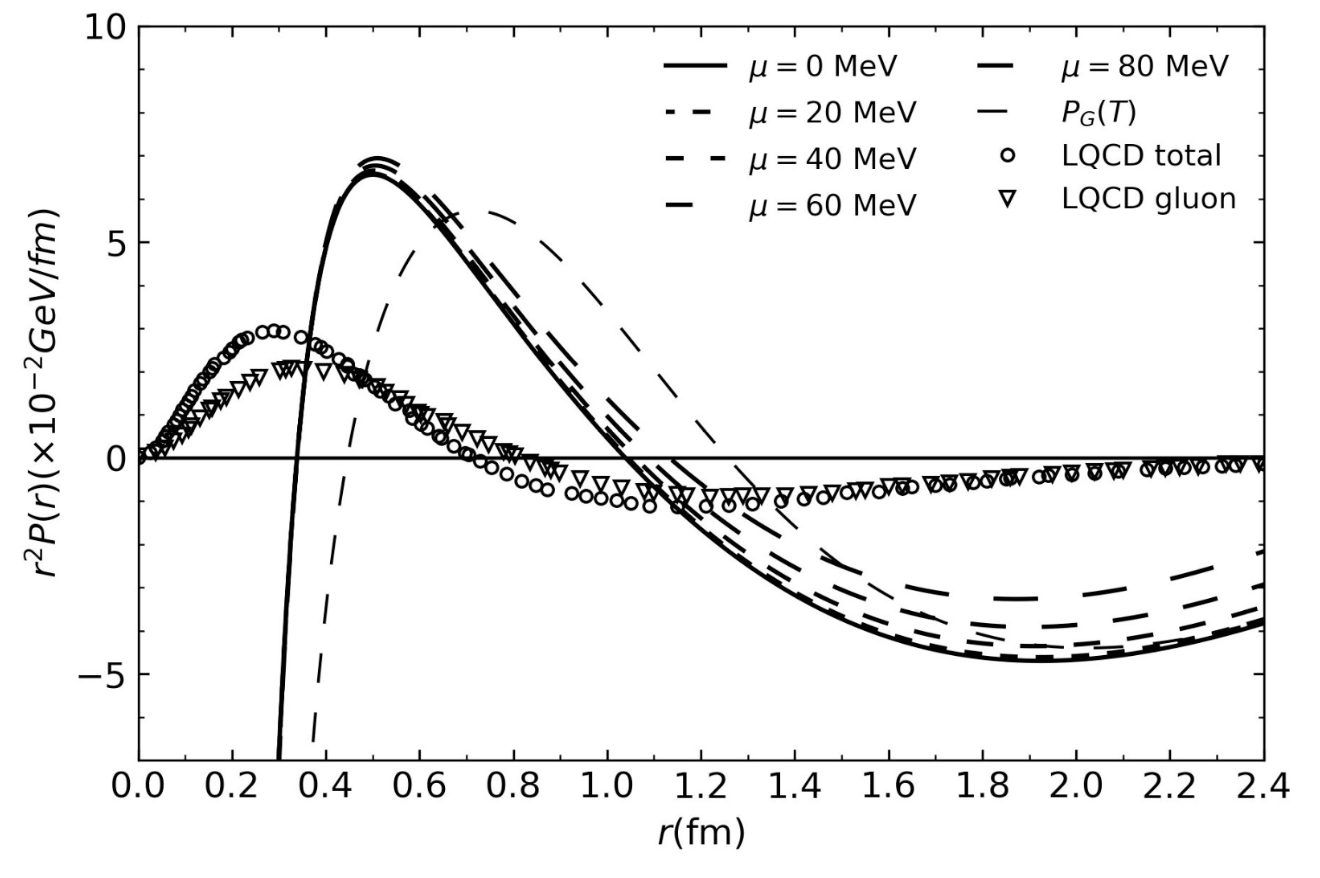
\includegraphics[width=0.58\textwidth]{./Images/MIT-BagModel.png}
    \caption[Comparación de presión radial con Lattice QCD]{\emph{Distribuciones radiales de presión \( r^2 P(r) \) obtenidas con el modelo Tsallis-MIT para distintos potenciales químicos \( \mu \) (líneas negras), comparadas con resultados de Lattice QCD de la referencia~\cite{shanahanPressureDistributionShear2019}. Los círculos representan la presión total \( P_q \), y los triángulos invertidos la componente gluónica \( P_G \).}}
    \label{fig:Results_LQCD}
\end{wrapfigure}

Se observa un notable acuerdo cualitativo entre ambas aproximaciones en el rango \( r \lesssim 1.2\,\mathrm{fm} \), donde la presión repulsiva alcanza su máximo alrededor de \( r \approx 0.5\,\mathrm{fm} \). Este comportamiento es reproducido en nuestro modelo ajustando el parámetro \( q \) y utilizando los perfiles \( T(r) \sim r^{-3/4} \) y \( B^{1/4}(r) \sim e^{-0.2936r} \), desarrollados en el Capítulo~\ref{ch-ProtonBagParameters}.

\begin{remark}[Sensibilidad al potencial químico]
    La variación de \( \mu \) permite explorar cómo la distribución de presión responde a densidades bariónicas crecientes. A medida que \( \mu \) aumenta, la presión repulsiva en la región central crece ligeramente, mientras que la zona de presión negativa se intensifica, indicando mayor confinamiento.
\end{remark}

Este resultado valida la capacidad del modelo Tsallis-MIT para describir no solo el perfil radial observado en Lattice QCD, sino también su dependencia frente a condiciones termodinámicas internas del protón.

\section{Influencia del potencial químico en la presión total}

La figura~\ref{fig:TotalPressureTsallis} muestra la evolución de la presión radial ponderada \( r^2 P(r) \) para distintos valores de \( \mu \), manteniendo fijo el parámetro de Tsallis en \( q = 1.05 \). Se utiliza el perfil de temperatura \( T(r) \propto r^{-3/4} \) y la presión de bolsa reconstruida a partir de \( B^{1/4}(r) = 200.9\,e^{-0.2936r}\,\mathrm{MeV} \).

\begin{figure}
    \centering
    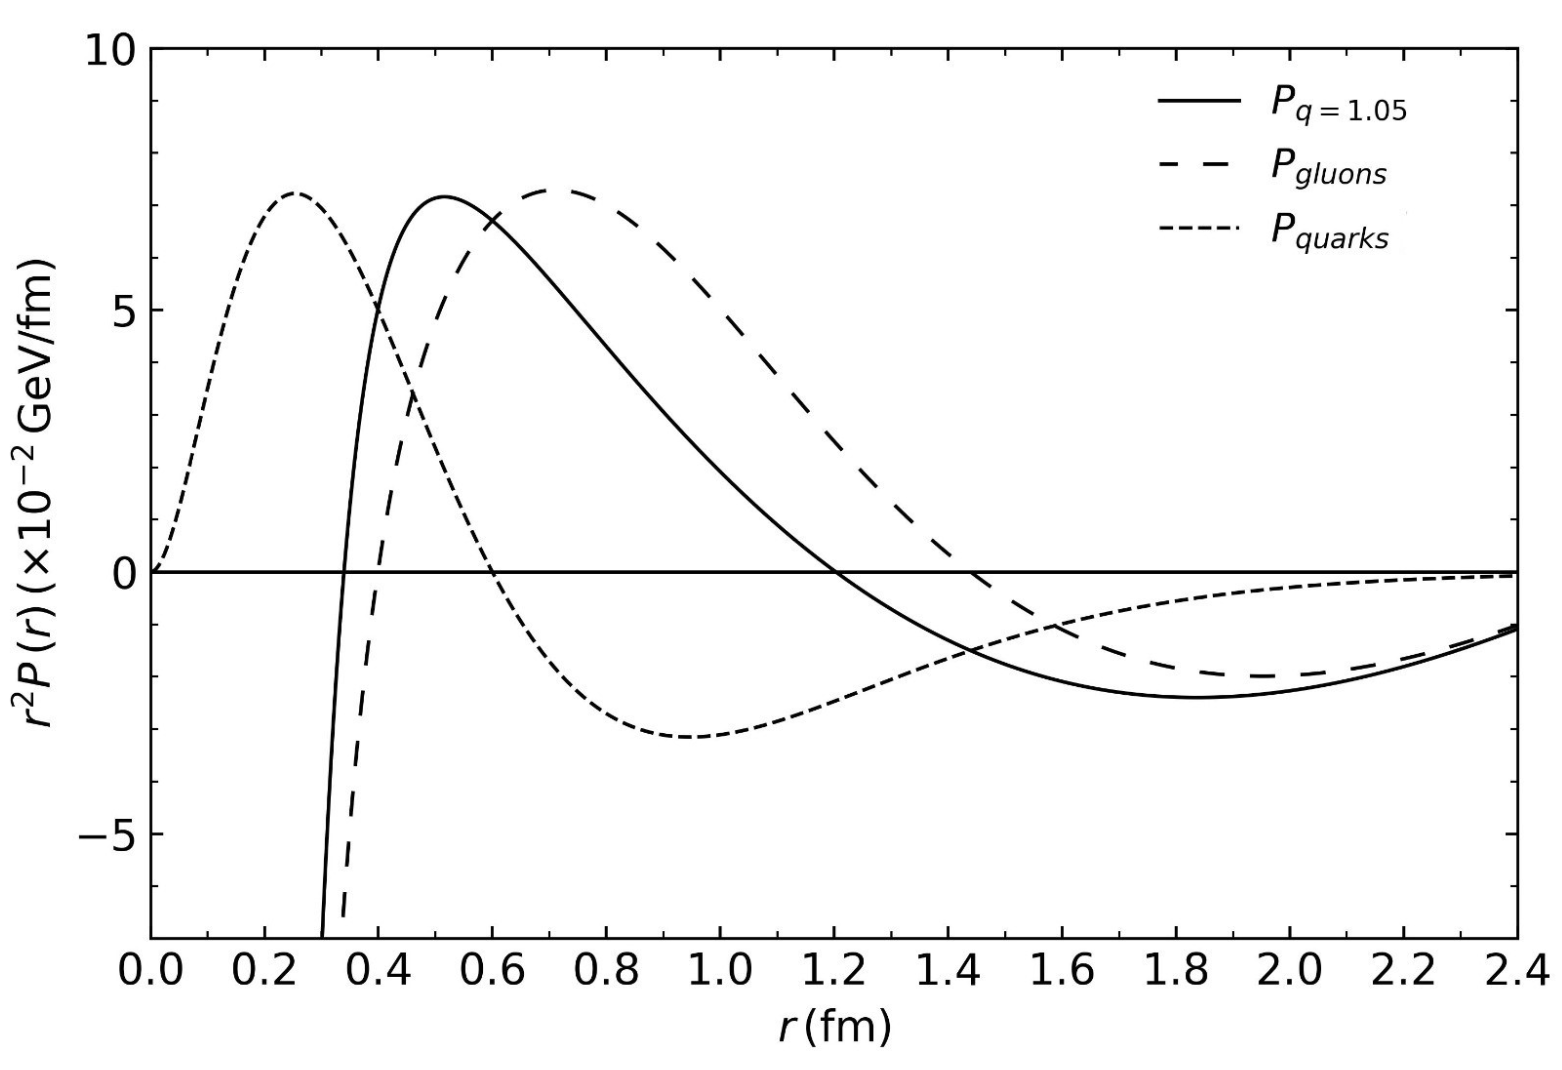
\includegraphics[width=0.58\textwidth]{./Images/PressureDistributionsTot-Q-G.png}
    \caption[Descomposición de presión radial]{\emph{Presión total \( P_q(r) \) (línea continua), presión gluónica \( P_G(r) \) (línea punteada larga) y presión de quarks \( P_Q(r) \) (línea punteada corta) para \( \mu = 100\,\mathrm{MeV} \) y \( q = 1.05 \). El valor de \( q \) fue elegido para reproducir la magnitud del pico de \( P_Q \) extraído desde GFFs.}}
    \label{fig:PressureDecompResult}
\end{figure}

Al incrementar el potencial químico:
\begin{itemize}
    \item La presión repulsiva cerca del centro se incrementa ligeramente.
    \item La transición hacia la región de presión negativa se vuelve más abrupta y profunda.
\end{itemize}

Este comportamiento refleja cómo el confinamiento se refuerza a mayores densidades bariónicas, en concordancia con expectativas de transiciones de fase a alta densidad.

El modelo Tsallis-MIT logra capturar esta dinámica sin necesidad de ajustes adicionales, destacando su versatilidad para describir la estructura interna del protón bajo diferentes condiciones.

\section{Extracción de la presión de gluones y validación de q}

La figura~\ref{fig:PressureDecompResult} muestra nuevamente las tres contribuciones a la presión radial ponderada \( r^2 P(r) \): la presión total \( P_q(r) \), la presión de quarks \( P_Q(r) \) extraída desde GFFs, y la presión de gluones \( P_G(r) = P_q(r) - P_Q(r) \). Este gráfico ya había sido presentado en el Capítulo~\ref{ch:TotalPandGluons} como parte del método de extracción, pero aquí lo utilizamos para validar el valor adoptado para el parámetro no extensivo \( q = 1.05 \).

Se observa que el valor \( q = 1.05 \) permite ajustar la presión total de forma que su pico coincida en magnitud con el de \( P_Q \), aunque desfasado en radio. Esto respalda la idea de que \( q \) encapsula los efectos efectivos del confinamiento, como se discutió en el Capítulo~\ref{ch-PhysicalMeaningQ}.

\begin{figure}
    \centering
    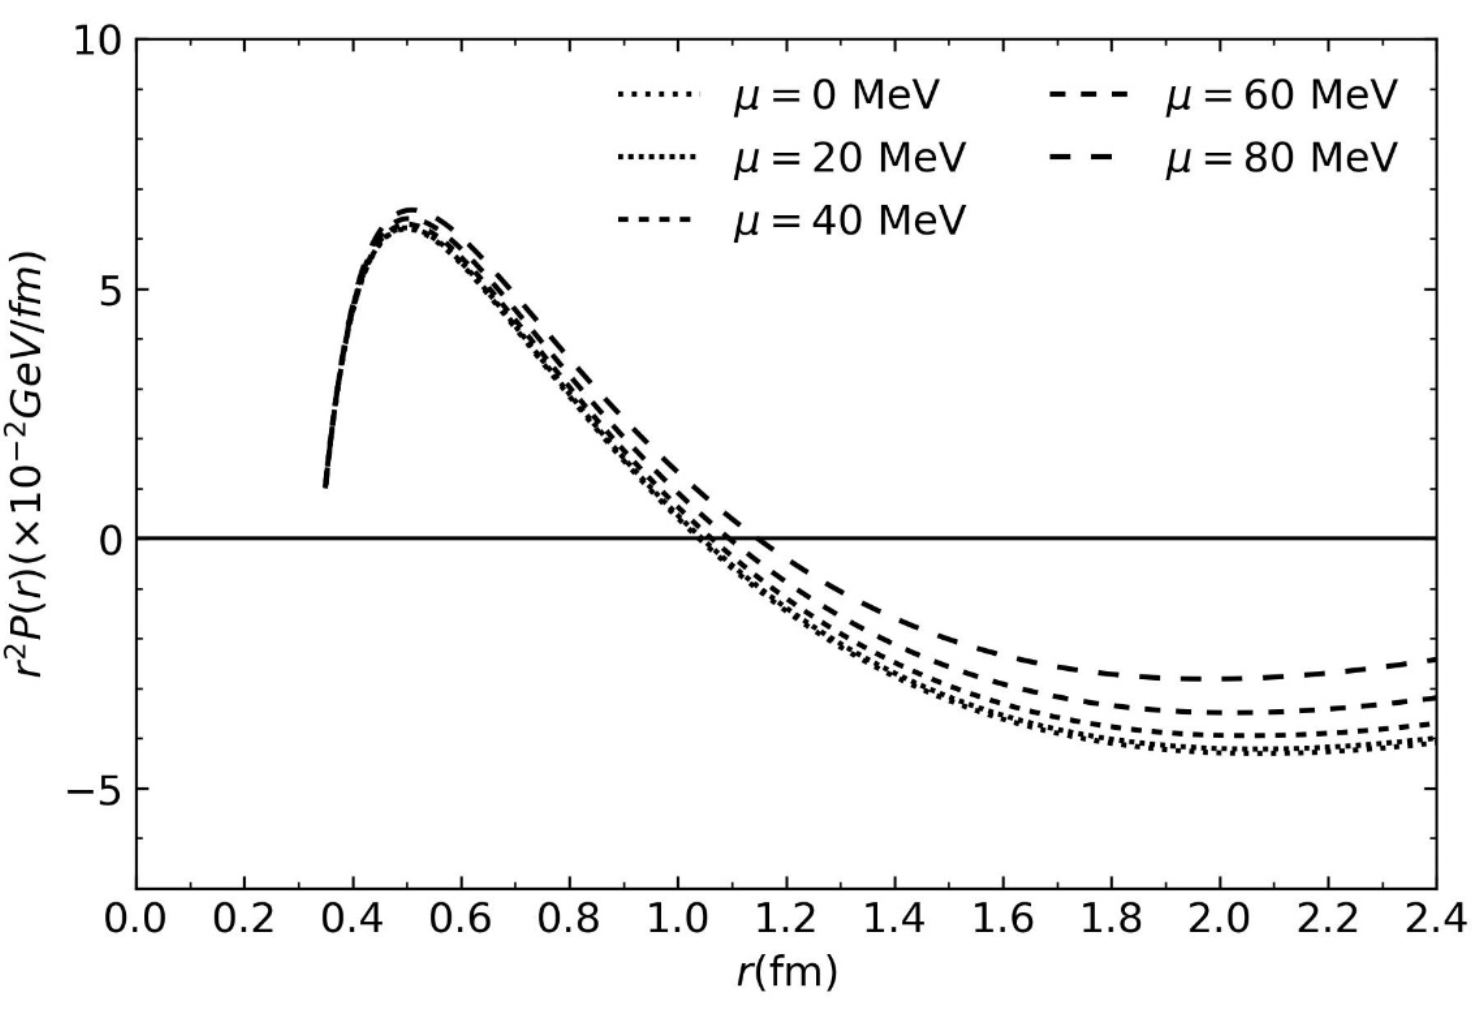
\includegraphics[width=0.58\textwidth]{./Images/TotalPressureTsallis.png}
    \caption[Efecto de \( \mu \) en la presión total radial]{\emph{Distribución radial ponderada \( r^2 P(r) \) obtenida con el modelo Tsallis-MIT para \( q = 1.05 \) y potenciales químicos \( \mu = 0, 20, 40, 60, 80\,\mathrm{MeV} \). La presión de bolsa se reconstruye a partir del ajuste \( B^{1/4}(r) = 200.9\,e^{-0.2936r}\,\mathrm{MeV} \).}}
    \label{fig:TotalPressureTsallis}
\end{figure}

\section{Reconstrucción de presiones equivalentes con distintos \( q \)}

Como se analizó en el Capítulo~\ref{ch-PhysicalMeaningQ}, es posible reconstruir perfiles de presión efectivos sin una presión de bolsa explícita, mediante la variación funcional del parámetro \( q \). En la figura~\ref{fig:B_reconstructed_combined}, se comparan dos distribuciones \( r^2 P(r) \) calculadas con valores distintos de \( q \) y sus correspondientes formas funcionales para \( B(r) \), mostrando que ambos enfoques reproducen perfiles similares.

\begin{figure}[H]
    \centering
    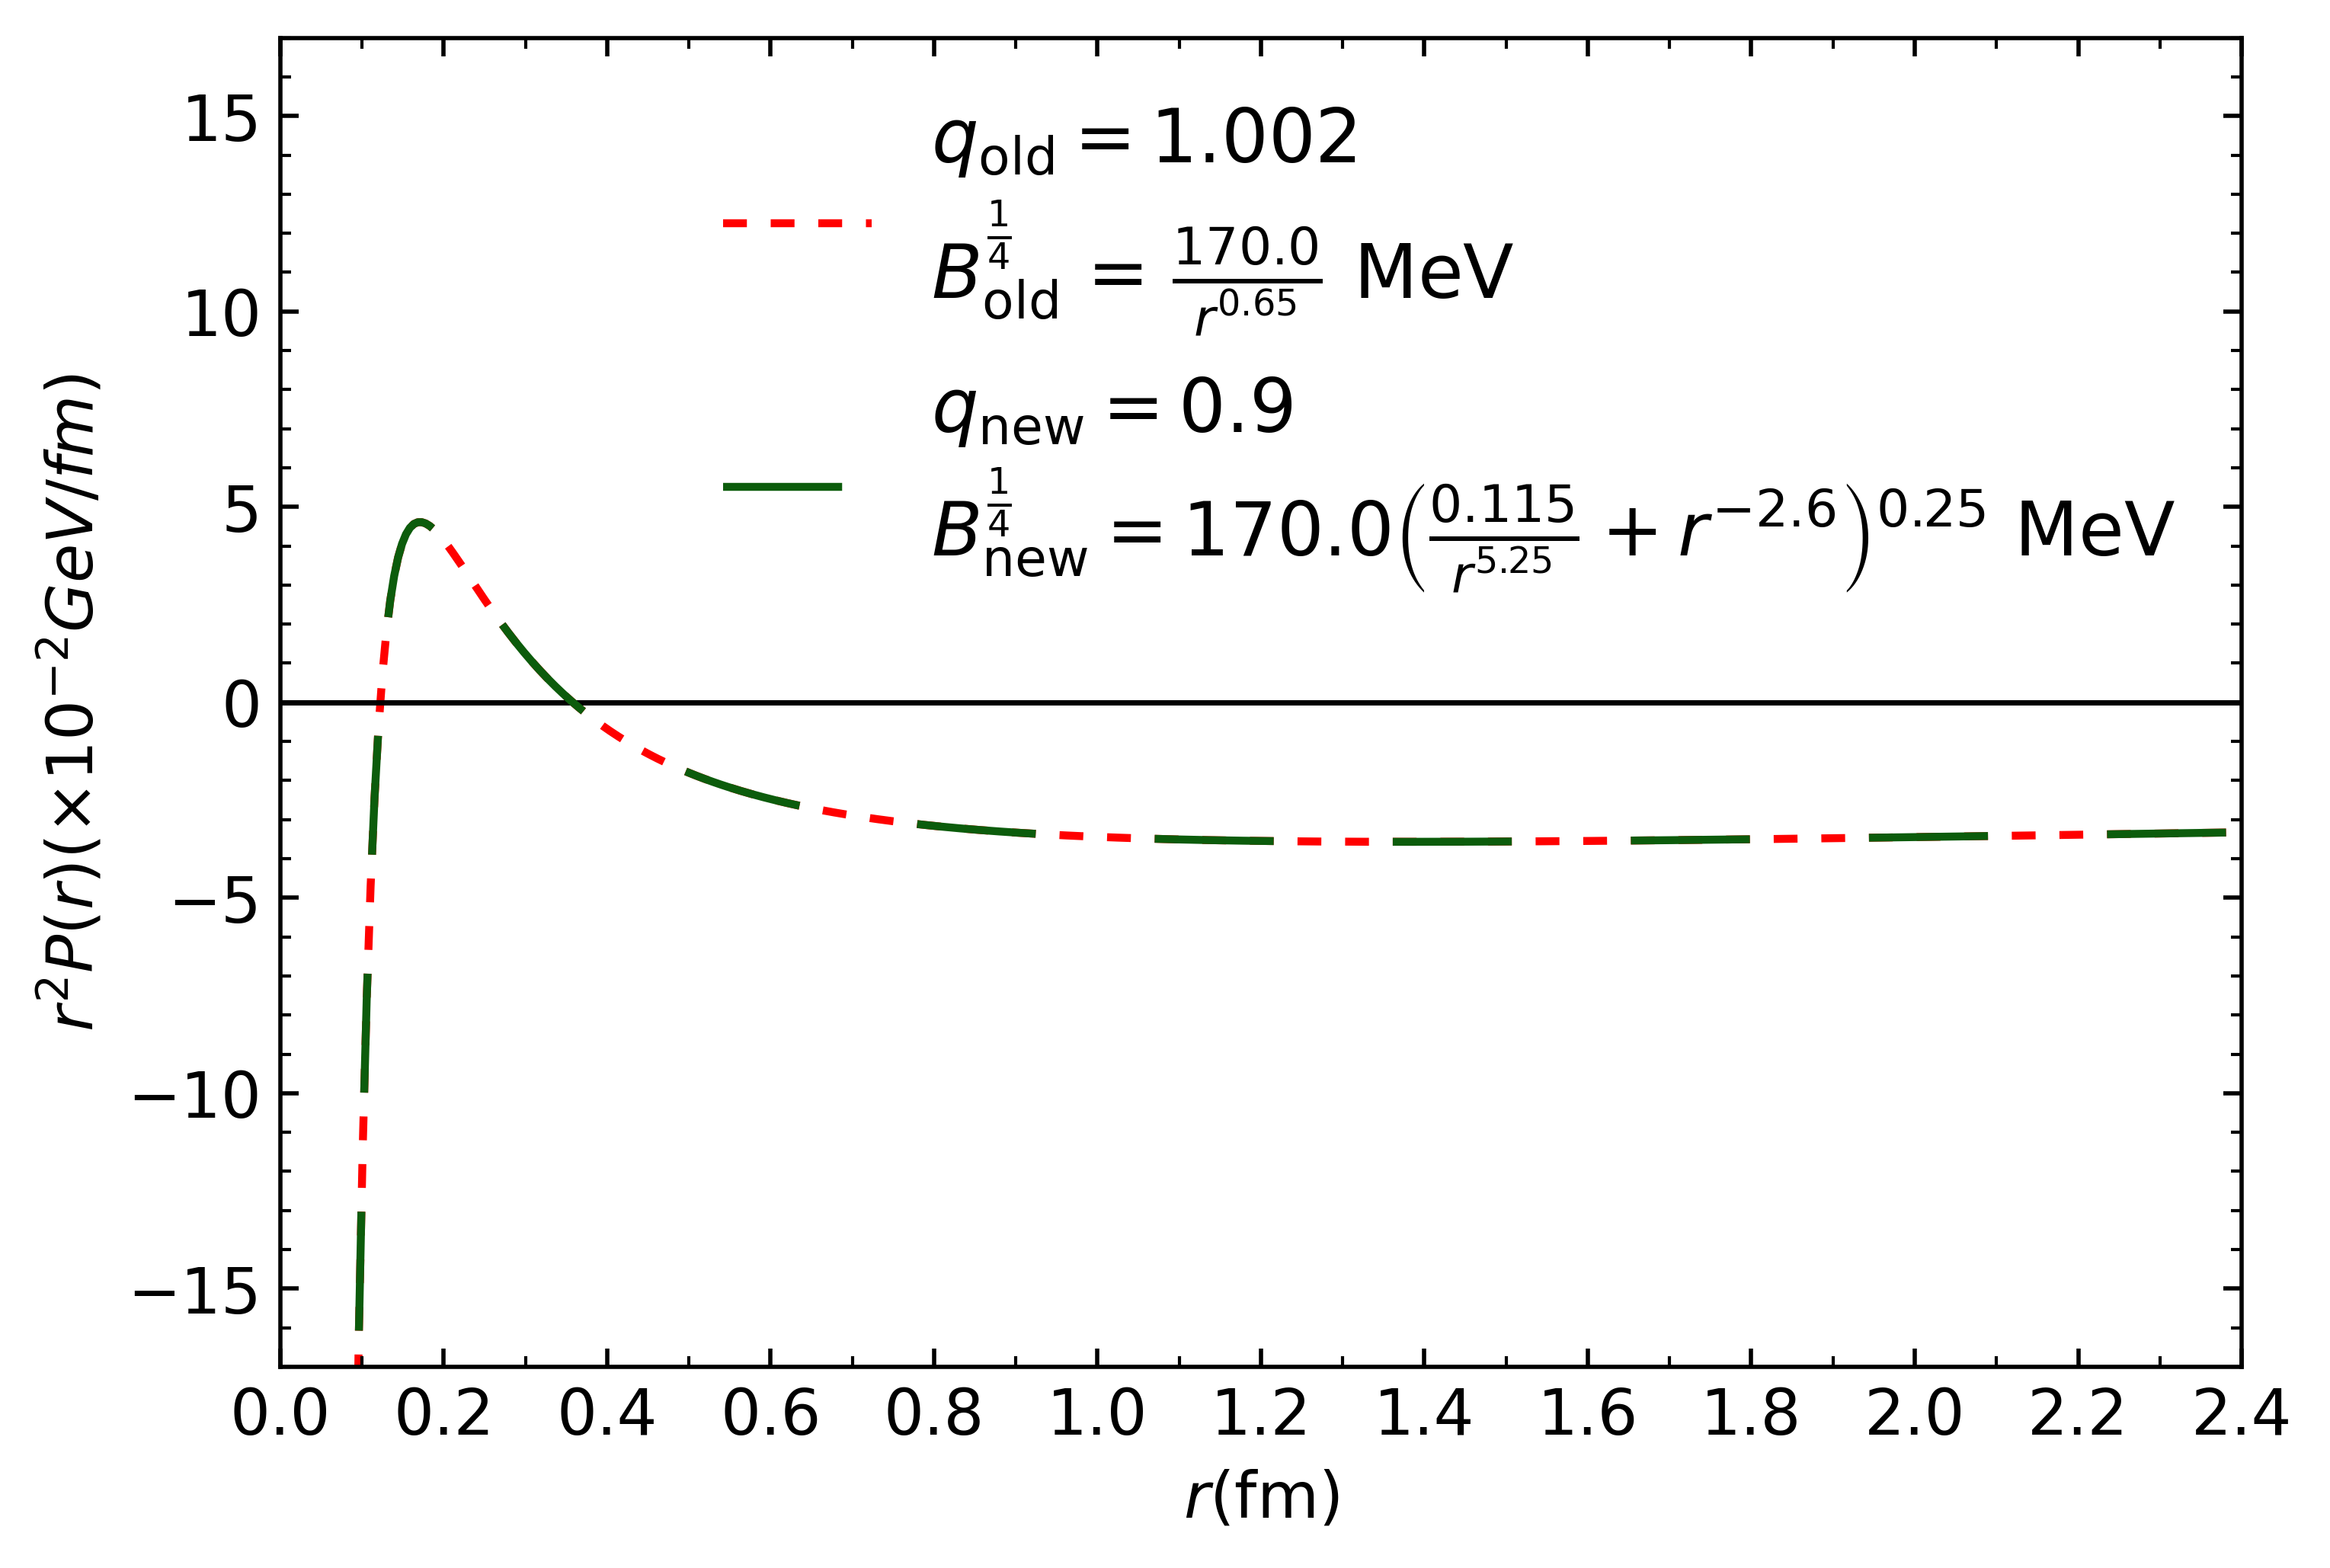
\includegraphics[width=0.75\textwidth]{./Images/Comparacion_B_old_new_combined.png}
    \caption[Comparación de perfiles con distintos \( q \)]{\emph{Comparación entre distribuciones \( r^2 P(r) \) obtenidas con \( q = 1.002 \) y una forma tradicional de \( B(r) \), y con \( q = 0.9 \) usando una forma funcional reconstruida. Ambos perfiles son compatibles en forma general, lo que respalda la hipótesis de que \( q \) puede absorber el efecto de confinamiento.}}
    \label{fig:B_reconstructed_combined}
\end{figure}

Este resultado fortalece la idea de que \( q \) puede interpretarse como un parámetro dinámico que encapsula la física del confinamiento, y no solo como un modificador estadístico.

\section{Conclusiones generales}

\begin{itemize}
    \item Se construyó un modelo efectivo basado en la estadística de Tsallis acoplado al modelo de bolsa MIT, capaz de reproducir distribuciones de presión hadrónica consistentes con QCD en el retículo.
    \item La dependencia radial del parámetro \( q(r) \) permite reinterpretar el confinamiento como un fenómeno emergente asociado a correlaciones no extensivas, prescindiendo potencialmente de la presión de bolsa fija.
    \item La validez del modelo se verificó frente a resultados de Lattice QCD y mediante reconstrucción inversa de perfiles de presión.
    \item La sensibilidad del modelo al potencial químico sugiere posibles aplicaciones en materia densa o escenarios de transición de fase (neutron stars, heavy-ion collisions, etc.).
\end{itemize}

\begin{remark}[Perspectivas]
    Futuras investigaciones podrían integrar una evolución dinámica de \( q(r,t) \), explorar efectos de anisotropías, o conectar con observables experimentales más allá de GFFs.
\end{remark}

\section*{Perspectivas de trabajo futuro}

Durante el desarrollo de este trabajo, se exploró preliminarmente la posibilidad de extender el modelo Tsallis-MIT al cálculo de masas hadrónicas. La idea inicial consistió en reinterpretar la energía total del sistema, \( U_q(T,V) \), derivada de relaciones termodinámicas de Tsallis, como responsable directa de la masa del hadrón, igualándola a la energía de bolsa tradicional. Esta propuesta permitió visualizar un posible camino hacia un modelo de masas dependiente explícitamente del parámetro de no extensividad \( q \).

Sin embargo, dado que los perfiles de temperatura \( T(r) \) y volumen efectivo \( V(r) \) ya estaban determinados fenomenológicamente, el cálculo resultante para \( q \) se reducía a un simple ajuste algebraico, limitando el alcance predictivo de esta aproximación.

Una perspectiva de trabajo futuro interesante sería implementar técnicas de aprendizaje automático (Machine Learning) para inferir el valor óptimo de \( q \) directamente a partir de masas experimentales de hadrones. A partir de un conjunto sintético generado por la energía \( U_q(T,V,q) \), podría entrenarse un regresor que prediga \( q \) como función de propiedades hadrónicas conocidas (masa, radio, temperatura). Esto permitiría validar de forma estadística la viabilidad del modelo Tsallis-MIT para describir espectros de masas sin necesidad de ajustes manuales.

Adicionalmente, se podrían explorar modificaciones a la condición de frontera de los modos normales en el modelo de bolsa, incorporando deformaciones dependientes de \( q \) en la ecuación trascendental de confinamiento. Esta estrategia abriría la posibilidad de obtener un espectro de masas directamente no extensivo desde la cuantización de los modos.

Aunque estos enfoques no fueron implementados en el presente trabajo, representan rutas prometedoras para investigaciones futuras que integren de manera más profunda la estadística de Tsallis en la fenomenología hadrónica.

\section*{Palabras finales}

Este trabajo presentó una formulación extendida del modelo de bolsa para nucleones mediante el uso de estadística no extensiva de Tsallis, integrando de manera natural los efectos del confinamiento y la correlación de largo alcance. Más allá de los resultados numéricos y validaciones presentadas, este estudio busca abrir nuevas líneas de exploración en la descripción efectiva de la materia hadrónica. 

Queda como perspectiva futura el desarrollo de modelos dinámicos basados en \( q(r,t) \), así como su contraste directo con datos experimentales provenientes de dispersión profunda y colisiones de alta energía.

\vspace{1em}
\noindent
\textit{“En la frontera entre estadística y confinamiento, emergen nuevas formas de comprender la estructura de la materia.”}

% Tu idea de partida —reinterpretar la masa total del hadrón como una energía interna derivada de la estadística de Tsallis, utilizando relaciones termodinámicas como U_q = F_q + TS_q, es conceptualmente muy sólida. De hecho, es una de las formas más lógicas y físicamente coherentes de intentar integrar Tsallis al cálculo de masas dentro de un modelo de bolsa. Así que sí, tu concepción es válida como cierre de este análisis.

% Sin embargo, si quisieras llevarlo más allá, aquí van algunas ideas adicionales por si en el futuro quieres retomarlo:

% ⸻

% 🧠 1. Redefinir la energía total U_q como suma de contribuciones energéticas no extensivas

% En el modelo de bolsa, la masa se construye con varios términos:
% M_{\text{bag}} = \sum_i \omega_i + \frac{4\pi}{3} R^3 B + \text{ZPE} + \Delta E

% Podrías intentar reinterpretar cada una de estas contribuciones como salidas de un sistema no extensivo:
% 	•	Las \omega_i como soluciones de un espectro modificado por q.
% 	•	El término de presión de bolsa como emergente de q, como ya haces.
% 	•	Incluso la energía de punto cero como una función efectiva de q, si se explora desde un enfoque cuántico deformado.

% Esto implicaría reescribir todo el modelo de bolsa en términos de Tsallis, lo cual es ambicioso, pero sería un gran paper teórico.

% ⸻

% 📊 2. Entrenar un modelo de ML para predecir q a partir de la masa hadrónica

% Dado que ya tienes:
% 	•	Las masas experimentales.
% 	•	Las expresiones de energía U_q(T, V, q) y los valores de T y V.

% Podrías generar un conjunto sintético de valores (T, V, q) \to M_q con la ecuación de Tsallis y luego ajustar un regresor inverso tipo scikit-learn para predecir q a partir de una masa dada.

% Esto te permitiría inferir cuál sería el valor de q necesario para reproducir M_{\text{exp}} sin depender de una forma funcional exacta, solo usando los datos. Puede no ser interpretativamente profundo, pero sí predictivamente útil.

% ⸻

% 🧪 3. Introducir un factor de deformación q en la ecuación trascendental de los modos

% La ecuación que resolviste:
% \tan x_{n\kappa} = \frac{x_{n\kappa}}{1 - mR - \sqrt{x_{n\kappa}^2 + (mR)^2}}
% podría modificarse incluyendo q como deformador de la condición de frontera, por ejemplo, en la raíz cuadrada como:
% \sqrt{x^2 + (mR)^2} \longrightarrow \sqrt{x^2 + (mR)^2} \cdot f(q)
% donde f(q) \to 1 cuando q \to 1. Así obtienes un espectro \omega_n(q), lo que te da acceso a calcular masas directamente modificadas por q.

% ⸻

% ✍️ ¿Y entonces?
% 	•	¿Vale la pena agregar esto ahora? → No necesariamente, ya tienes una idea clara y cerrada.
% 	•	¿Vale la pena mencionarlo como trabajo a futuro? → ¡Definitivamente sí!

% Te puedo redactar un \begin{remark}[Trabajo futuro] o \section*{Ideas complementarias} para agregarlo si gustas. ¿Te gustaría?